\section{Graf jadier}

V tejto časti popíšeme ako z jadier korekcie zostavíme kvázi de Bruijnov graf pre jedno čítanie. Vstupom je zoznam prekrytí medzi čítaniami a pre každé prekrytie aj zoznam jeho jadier. Výstupom je graf, v ktorom jadrá sú vrcholy a hrany sú medzi jadrami, ktoré sa prekrývajú. Príklad takého grafu je na obrázku \ref{fig:pseudo_debruijn}.

\begin{figure}
    \centering
    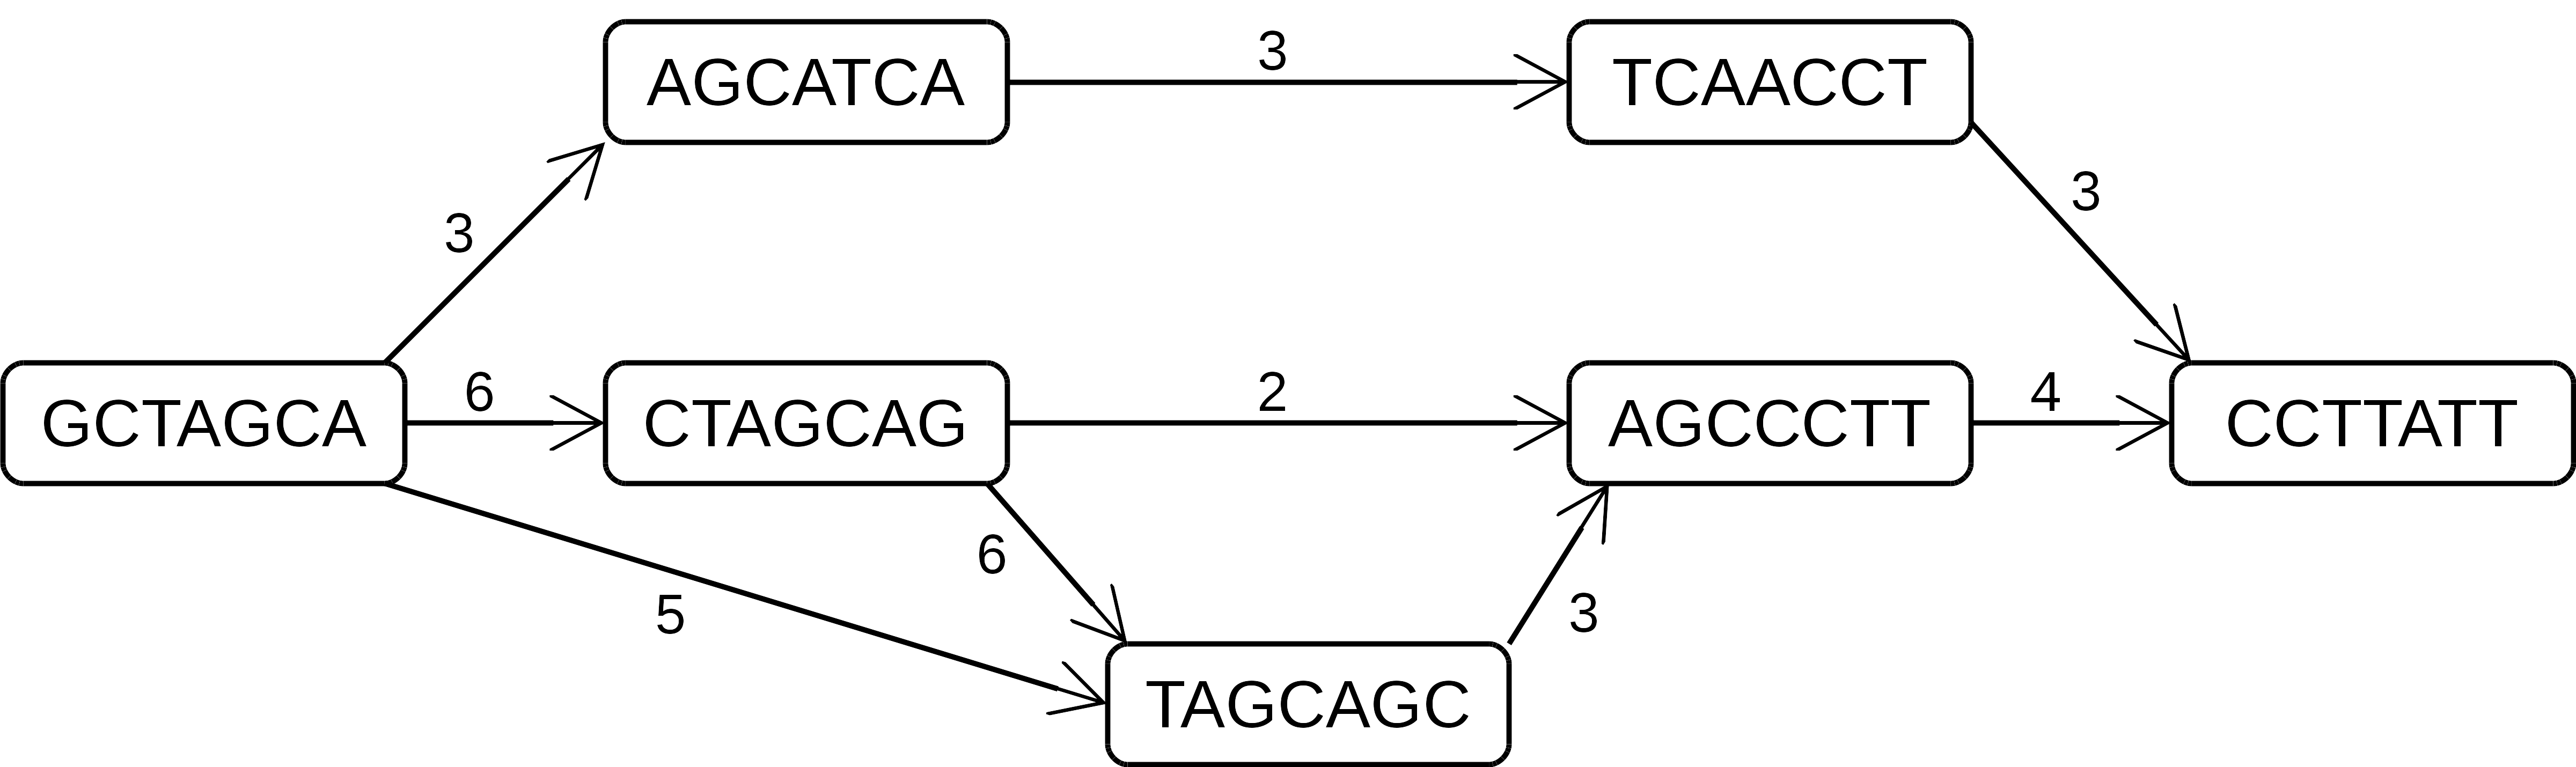
\includegraphics[width=0.8\textwidth]{images/pseudo_debruijn.png}
    \caption{Ukážka grafu jadier korekcie}
    \label{fig:pseudo_debruijn}
\end{figure} 

Začneme vytvorením zoznamu všetkých jadier z opravovaného čítania a z čítaní, ktoré sa s ním prekrývajú. Aby sme sa vyhli problémom súvisiacim so vzájomným prekrývaním jadier, rozbijeme dlhšie jadrá na postupnosť prekrývajúcich sa jadier pevnej dĺžky. Je vhodné použiť tú istú dĺžku ako bola minimálna dĺžka jadra v predchádzajúcej podkapitole. Pre každé jadro si algoritmus pamätá, či pochádza z opravovaného čítania, odhadovanú pozíciu a jej prislúchajúcu sekvenciu. Jadrá z opravovaného čítania budeme označovať silné. Tým, že jadrá sú pevnej dĺžky, ktorá neprekročí hodnotu 32, môžeme sekvencie reprezentovať ako celé čísla. V prípade, že prekrývajúce čítanie je z opačného vlákna, do zoznamu pridávame jadrá s obrátenou komplementárnou sekvenciou.

\subsection{Odhadovanie pozície jadra}

Na rozdiel od nástroja LoRDEC, kde sa de Bruijnov graf zostavoval z iných čítaní, máme k dispozícii informáciu o pozícii jadier v rámci ich čítaní. Čím presnejšie odhadneme pozície jadier na opravovanom čítaní, tým prísnejšie podmienky môžeme nastaviť pri vytváraní hrán v grafe. 

Pre silné jadrá je pozícia jasne určená. V prípade jadier z prekrývajúcich sa čítaní môžu nastať dve situácie:

\begin{enumerate}[label={S.\arabic*}]
\item \label{jadro_medzi_dvomi_silnymi} Jadro sa nachádza medzi dvomi silnými jadrami
\item \label{jadro_medzi_silnym_a_okrajom_citania} Jadro sa nachádza na okraji čítania a silné čítanie má len na jednej strane.
\end{enumerate}

Pri odhadovaní pozície jadier prekrývajúceho sa čítania si do vyvažovaného stromu pre všetky silné jadrá uložíme dvojice (pozícia v prekrývajúcom sa čítaní, pozícia v opravovanom čítaní). Túto dátovú štruktúru potom použijeme na rozlíšenie medzi \ref{jadro_medzi_dvomi_silnymi} a \ref{jadro_medzi_silnym_a_okrajom_citania}. V prípade \ref{jadro_medzi_dvomi_silnymi} sa na vypočítanie pozície jadra použije priemer posunov najbližších silných jadier naľavo a napravo. V prípade \ref{jadro_medzi_silnym_a_okrajom_citania} použijeme len posun najbližšieho silného jadra. Názorná ukážka je na obrázku \ref{fig:odhadovanie_pozicie}. Červenou sú označené silné jadrá, zelenou je označený príklad situácie \ref{jadro_medzi_dvomi_silnymi} a modrou \ref{jadro_medzi_silnym_a_okrajom_citania}. Jadrá, ktoré sa zobrazia mimo opravovaného čítania, ďalej nebudeme brať do úvahy.

\begin{figure}
    \centering
    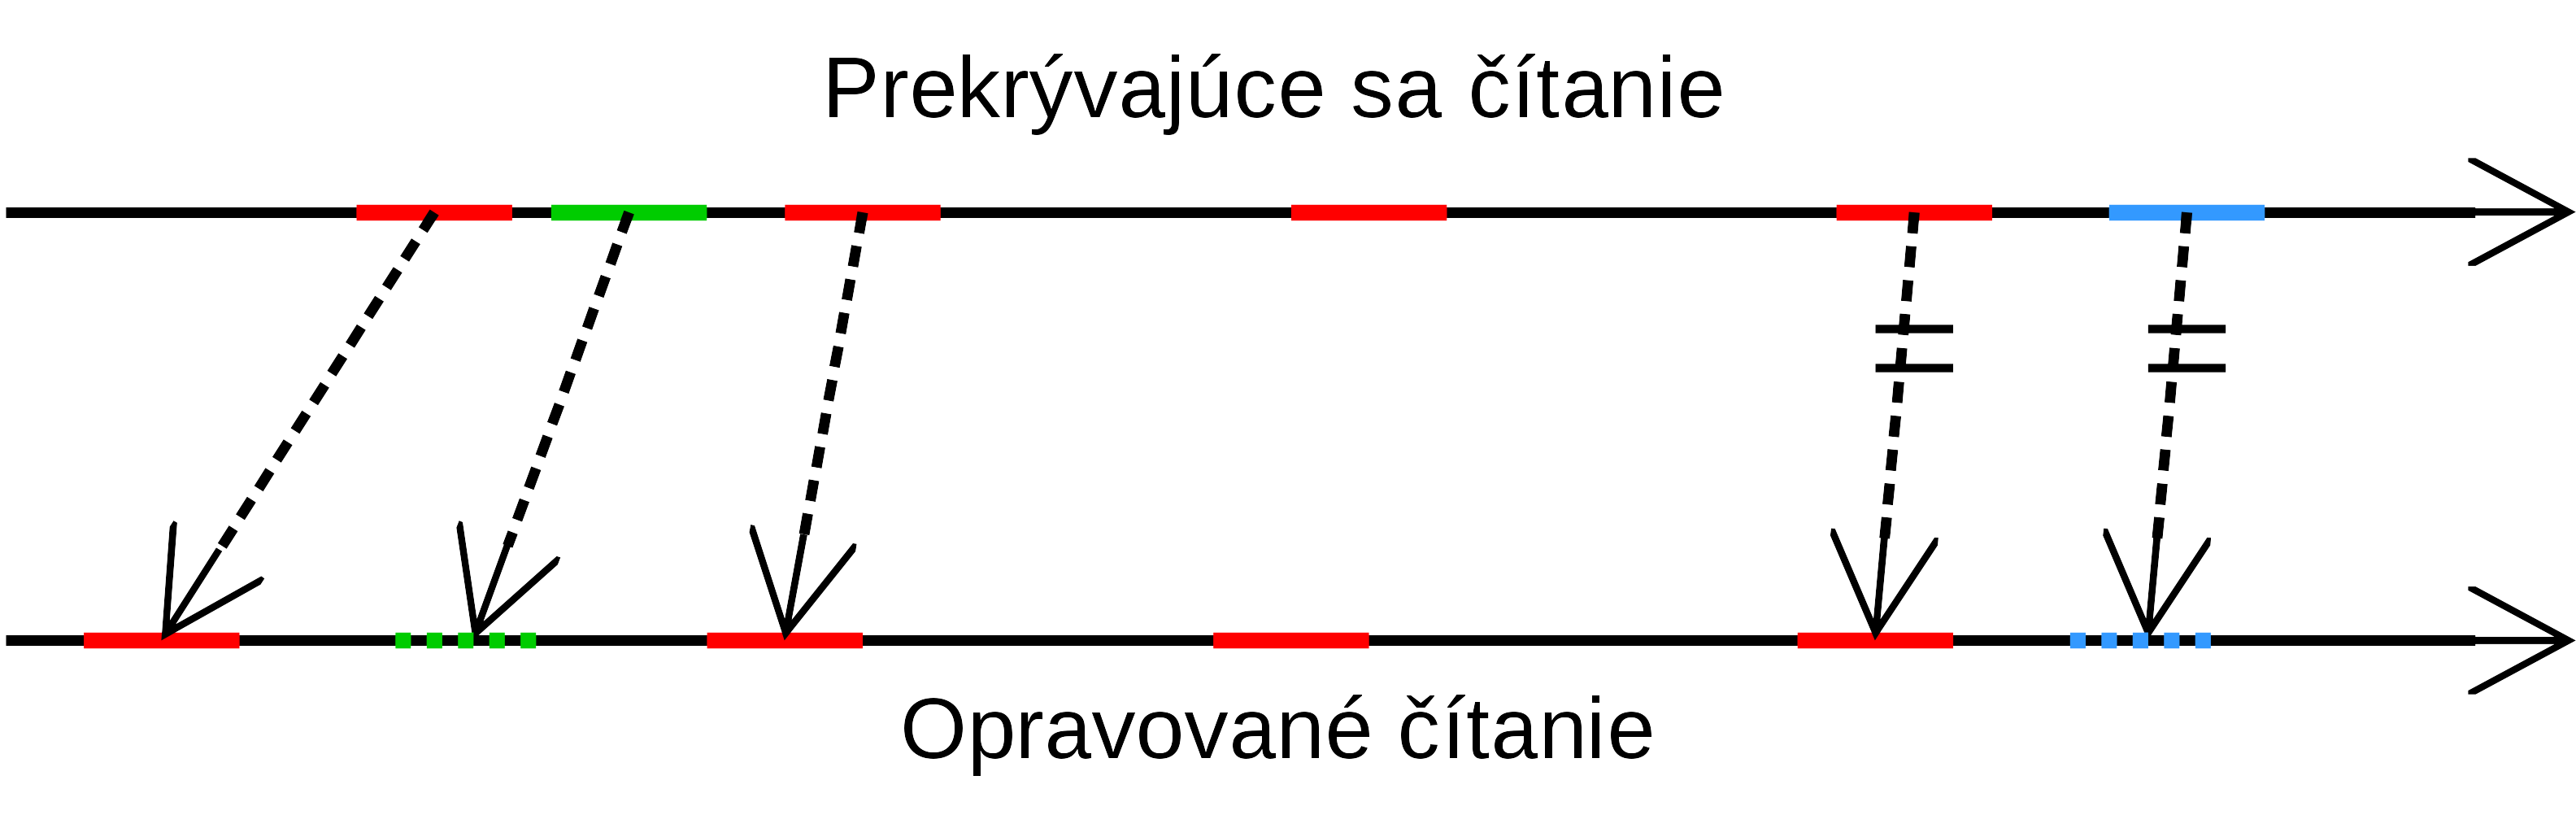
\includegraphics[width=0.8\textwidth]{images/odhadovanie_pozicie.png}
    \caption{Ukážka odhadovania pozícií jadier}
    \label{fig:odhadovanie_pozicie}
\end{figure} 

\subsection{Odstraňovanie duplikátov}

Mnohé správne jadrá sa v zozname vyskytujú viackrát. Tieto duplikáty by v grafe umožnili vytvárať až exponenciálne veľa rôznych ciest, ktoré by indukovali rovnaké sekvencie. Riešením tohto problému je spájanie jadier s rovnakou sekvenciou a blízkou očakávanou pozíciou do jedného. Výsledné jadrá považujeme za silné, ak aspoň jedno z pôvodných bolo silné. Očakávaná pozícia výsledného jadra je priemer očakávaných pozícií pôvodných jadier. Dosiahneme to usporiadaním zoznamu podľa sekvencie (celé číslo) a podľa očakávanej pozície a následne jedným prechodom cez zoznam. 

\subsection{Prekrytia jadier}

Hrany v generovanom grafe sú dané prekrytiami sekvencií jadier. V de Bruijnovom grafe sa hrany štandarne vytvárajú len ak majú prekrytie na $k - 1$ bázach, kde $k$ je dĺžka sekvencie vrchola a ak sa sekvencie niekde vyskytli za sebou vo vstupných dátach. V našom prípade sa nemôžeme spoliehať, že by na každej pozícii opraveného čítania začínalo nejaké jadro korekcie, čiže musíme povoliť aj prekrytia menšie ako $k - 1$. Druhú podmienku tiež musíme vypustiť, lebo je pre nás nevyhnutné prechádzať cez jadrá pochádzajúce z rôznych čítaní. 

Algoritmus osobitne rieši prekrytia rôznych dĺžok. Pri získavaní prekrytí dĺžky $l$ vytvorí zoznam všetkých prefixov a sufixov sekvencií jadier dĺžky $l$. Sekvencie máme reprezentované celými číslami, takže vytváranie prefixov a sufixov je realizovateľné pomocou bitového posunu, resp. bitovej operácie AND s vhodnou maskou. Tu opäť využijeme vhodné usporiadanie zoznamu a to podľa čísla sekvencie a bitu \{sufix, prefix\}. V usporiadanom zozname v rámci jednej skupiny rovnakých sekvencii program vytvorí hranu medzi všetkými dvojicami sufix -- prefix. Vytváranie hrán z jednej skupiny je znázornené v tabuľke \ref{table:prekrytia_jadier}.

\begin{table}
    \begin{subtable}{.5\linewidth}
        \centering
\begin{tabular}{ c }
    \verb|      ...     | \\
	\hline
	\color{red}     \verb|ACTCTACGCGT   | \\
	\color{green}   \verb|CGCCTACGCGT   | \\
	\color{blue}    \verb|TCACTACGCGT   | \\
	\color{cyan}    \verb|   CTACGCGTACC| \\
	\color{magenta} \verb|   CTACGCGTCTA| \\
	\hline
    \verb|      ...     | \\
\end{tabular}
        \caption{}
        \label{subtable:skupina_suf_pref}
    \end{subtable}
    \begin{subtable}{.5\linewidth}
        \centering
        \begin{tabular}{ c c }
        	\hline
           	Z & Do \\ \hline \hline
           	 \color{red}    \verb|ACTCTACGCGT| & \color{cyan}    \verb|CTACGCGTACC| \\
           	 \color{red}    \verb|ACTCTACGCGT| & \color{magenta} \verb|CTACGCGTCTA| \\
           	 \color{green}  \verb|CGCCTACGCGT| & \color{cyan}    \verb|CTACGCGTACC| \\
           	 \color{green}  \verb|CGCCTACGCGT| & \color{magenta} \verb|CTACGCGTCTA| \\
           	 \color{blue}   \verb|TCACTACGCGT| & \color{cyan}    \verb|CTACGCGTACC| \\
           	 \color{blue}   \verb|TCACTACGCGT| & \color{magenta} \verb|CTACGCGTCTA| \\
           	 \hline
        \end{tabular}
        \caption{}
        \label{subtable:vytvorene_hrany}
    \end{subtable}
    \caption{Sekvencie v jednej skupine rovnakých sufixov a prefixov (a) a hrany vytvorené medzi jadrami (b)}
    \label{table:prekrytia_jadier}
\end{table}

\subsubsection{Heuristiky}

Ak by sme nijako neobmedzili počet hrát vychádzajúcich z jedného vrcholu v grafe, v priemere by ich bolo viac ako $|V|/4$. Išlo by prevažne o hrany s prekrytím dĺžky 1 a 2 a vačšina z nich by bola čisto náhodná. Jedna možnosť, ako sa s tým vysporiadať, je nastaviť fixnú minimálnu dĺžku prekrytia $m$. Miestam v čítaní, ktoré sú dobre pokryté jadrami korekcie, by to nijako neuškodilo. Algoritmus aj tak uprednostňuje hrany s dlhším prekrytím. Horšie by dopadli úseky, kde sú jadrá rozmiestnené riedko. Čítanie by sa v týchto miestach buď vôbec nedalo z jadier vyskladať alebo by sa použila iná nesprávna cesta. Ďalšia možnosť je obmedziť počet hrán vychádzajúcich z jedného vrcholu s tým, že by zostalo len $n$ hrán s najdlhším prekrytím. Myšienkou za touto heuristikou je, že ak zo správneho jadra $x$ vieme preskočiť s veľkým prekrytím na jadro $y$ a s malým prekrytím na jadro $z$, potom existuje aj hrana (alebo postupnosť hrán) z $y$ do $z$. %Vhodnú kombináciu parametrov $m$ a $n$ sme experimentálne zistili a popísali v nasledujúcej kapitole.

Pri obmedzovaní počtu hrán vieme využiť aj informáciu o očakávanej pozícii jadier korekcie. Hranu medzi dvomi jadrami vytvoríme len v prípade, že ich očakávaná pozícia je dostatočne blízko. Vplyv týchto troch heuristických metód na kvalitu korekcie sme otestovali a výsledky sú uvedené v nasledujúcej kapitole.